\documentclass[a4paper,10pt]{article}
\usepackage[utf8]{inputenc}
\usepackage[french,english]{babel}
\usepackage{mathptmx}
\usepackage{float}
\usepackage{graphicx}
\usepackage{url}
\usepackage{color}

\setlength{\parindent}{0em}
\setlength{\parskip}{1em}
\addtolength{\hoffset}{-4em}
\addtolength{\textwidth}{8em}
\addtolength{\voffset}{-6em}
\addtolength{\textheight}{12em}

\begin{document}
\thispagestyle{empty}

{\bf
	\emph{Fast-Marching} Hamiltonien avec conditions aux limites mixtes
}

{\bf Encadrants}:\\
Marie d'Autume \verb+<mariedautume@gmail.com>+ \\
Enric Meinhardt-Llopis \verb+<enric.meinhardt@ens-paris-saclay.fr>+

{\bf Description}\\
Un des problèmes les plus anciens et les plus vénérables des mathématiques est
le calcul du volume d'un tas de sable~\cite{archimedes,monge}.  La théorie
moderne de l'intégration réduit ce problème au problème du calcul de la forme
du tas.  L'objectif de ce stage est de proposer une méthode pour
calculer le volume à partir d'une~\cite{horn} ou de plusieurs~\cite{woodham}
photographies aériennes du tas.
Plus concrètement, nous utiliserons la méthode de \emph{Fast-March} Hamiltonien
de Mirebeau~\cite{mirebeau} pour résoudre numériquement l'équation de ``Shape
From Shading'' associée au problème.
%, sans forcément passer par un modèle 3D complet.

\begin{figure}[H]
	\begin{center}
		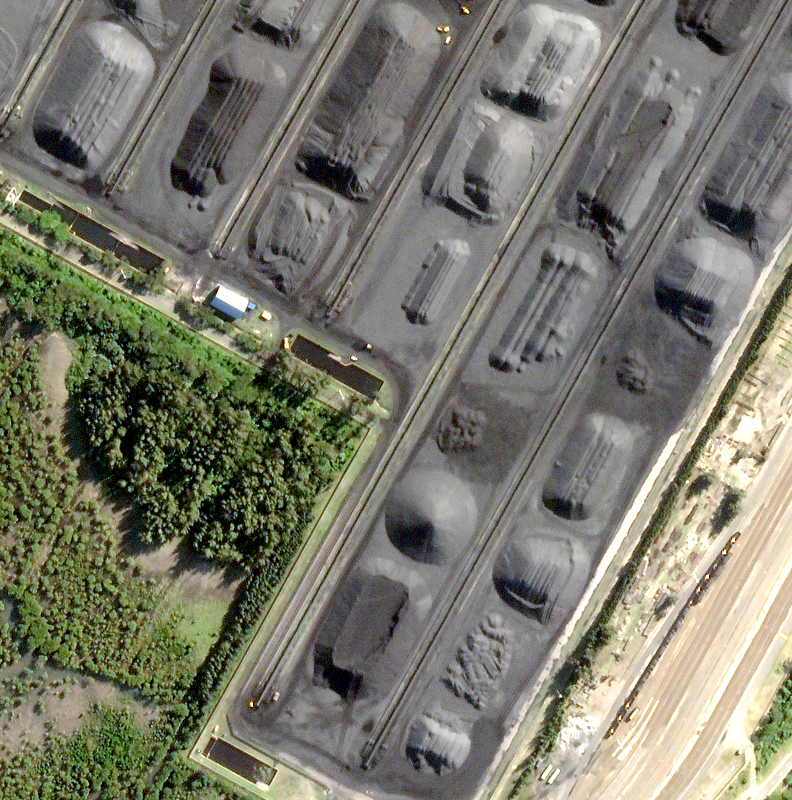
\includegraphics[width=0.49\textwidth]{f/sv.png}
	\end{center}
    \vspace{-1.5em}
	\caption{
		Photographie satellite d'un ensemble de tas de charbon près
		d'une raffinerie.  L'objectif du stage consiste à faire un
		programme qui calcule le volume de la réserve à partir d'une
		image comme celle-ci.
	}
\end{figure}

Une formulation simple de ce problème est fournie par le modèle
d'\emph{illumination Lambertienne}, qui donne une relation entre l'image
observée~$I(x,y)$ et la surface du tas~$z=u(x,y)$
\[
	I(x,y) = \alpha\, \frac{au_x+bu_y+c}{
	\sqrt{u_x^2+u_y^2+1}}
\]
où~$\alpha$ est l'albédo de la surface et~$(a,b,c)$ la direction du soleil, qui
sont des paramètres à priori connus.  L'objectif est donc de
calculer~$\mathbf{vol}(u)=\int_{\Omega}u$ à partir d'une condition aux
limites~$u|_{\partial\Omega}$ donnée.  Cette relation est une EDP non-linéaire d'ordre~$1$
qui n'aura à priori pas de solution unique.  On étudiera donc des restrictions
de la notion de solution (solutions de viscosité~\cite{viscosite}) et des méthodes pratiques de
calcul de cette solution (\emph{fast-marching} à partir de la condition de
bord~\cite{mirebeau}).
Le but final étant de développer et décrire une méthode complète qui passe de
l'image~$I$ au volume~$\mathbf{vol}(u)$ en choisissant automatiquement des
conditions de bord appropriées.
%On considérera
%l'effet de ces approximations sur la valeur finale de
%$\mathbf{vol}(u)$, qui en serait dans l'idéal une quantité invariante.

%Au cours du stage, le groupe d'élèves lira les articles clés sur le sujet, qui
%font appel à des connaissances d'algèbre linéaire, équations différentielles et
%traitement d'images.
%Les méthodes numériques proposées seront enfin mises en
%œuvre avec un langage de programmation choisi par les étudiants (\emph{Python,
%Matlab, ou C/C++}).

    \vspace{-1.5em}
\renewcommand{\refname}{\normalsize Références}
%
\begin{thebibliography}{99}
\vspace{-1em}
{\footnotesize
\bibitem{archimedes}
	Archimède, {\it De la sphère et du cylindre}, 225 av. J.-C.

\bibitem{monge}
	G.~Monge, {\it Sur la théorie des déblais et des remblais}.
		Mém. de l’acad. de Paris, 1781

\bibitem{horn}
	B.K.P.~Horn, {\it Shape from Shading: a Method for Obtaining the Shape
		of a Smooth Opaque Object from One View.}
		MIT Technical Report, 1970

\bibitem{woodham}
	R.J.~Woodham, {\it Photometric method for determining surface
		orientation from multiple images.} Optical engineering, 1980

\bibitem{viscosite}
E. Rouy, A. Tourin
{\it A Viscosity Solutions Approach to Shape-From-Shading }
SIAM Journal of Numerical Analysis, 1992

\bibitem{mirebeau}
	J.-M. Mirebeau, J. Portegies,
	{\it Hamiltonian Fast Marching: A Numerical Solver for Anisotropic and
Non-Holonomic Eikonal PDEs}
	IPOL, 2019

%\bibitem{retinex} Land, E. H., and McCann, J. J. Lightness and Retinex Theory. Journal of the Optical Society of America, 1971.
%
%\bibitem{shepard} Shepard, D. A two-dimensional interpolation function for irregularly-spaced data. ACM national conference, 1968.
%
%%\bibitem{ssao} Bavoil, L. and Sainz, M.. Screen space ambient occlusion. NVIDIA developer information, 6, 2008.
%
%\bibitem{unser} Q. Sun, and M. Unser. Left-inverses of fractional Laplacian and sparse stochastic processes. Advances in Computational Mathematics, 2012.
%
%%\bibitem{whitening} Goldstein, A., and Fattal, R. Blur-Kernel Estimation from Spectral Irregularities. In Computer Vision – ECCV 2012, (2012).
}
\end{thebibliography}

%{\bf old seamless cloning text}
%
%\noindent  \emph{Seamless image cloning} (copier-et-coller sans couture) est un outil important pour l'édition d'images et video
%qui consiste à copier un morceau d'une image source et le coller dans une image de destination de sorte de pas introduire 
%des artefacts visibles sur la frontière de la région modifiée.
%Le renommée méthode de \emph{poisson editing} (Perez et al. 2003) propose de résoudre ce problème
%par la minimisation d'une énergie définie sur le domaine à éditer $\Omega$ (de forme arbitraire)
% \[  \min_{f} \int_{\Omega} | \nabla f  - \mathbf{v} |^2  \mbox{    s.t.    }    f|_{\partial \Omega} = f^*|_{\partial \Omega},\] 
% où $f^*$ denote l'image cible et $\mathbf v$ sont des gradients obtenus a partir de l'image source $g$.
%%
%Lorsque $ \mathbf v = \nabla g$, la solution au problème de poisson editing peut être décrit en termes de
%la solution de l'équation de Laplace sur le domaine $ \Omega $ avec conditions de Dirichlet aux bords.
%Au cours \emph {d'Analyse Hilbertienne et de Fourier} nous avons vu que si le domaine est rectangulaire
%la solution a cette problème peut être calculée efficacement en utilisant la transformée de Fourier rapide.
%Par contre les algorithmes de résolution itératives utilises pour des domaines arbitraires sont généralement lents.
%
%La méthode de \emph{``convolution pyramids''}  récemment proposée  par Farbman et al. (2011) utilise un approche multi-échelle pour calculer des solutions approximatives de l'équation de Laplace de façon très efficace.
%Mais, même si l'algorithme est  simple dans la pratique, les auteurs reconnaissent que son comportement n'est pas entièrement comprise d'un point de vue théorique. 
%
%
%L'objective de cet stage est donc d'étudier l'algorithme de \emph{``convolution pyramids''} appliquée à la resolution de l'équation de Laplace avec conditions de Dirichlet aux bords, pour 
%%comprendre son fonctionnement, 
%identifier ses limites, et éventuellement caracteriser les circonstances dans lesquelles l'approximation obtenue est la pire.
%%Spécifiquement  nous sommes intéressés à la caractérisation des circonstances dans lesquelles l'approximation est la pire.
%Ceci demande réflexion et expérimentation. Durant le stage, le groupe d’élèves lira les articles clés sur le sujer qui leur seront fournis, et qui font appel à des connaissances d’analyse fonctionnelle, calcul variationel, et à pas mal d’effort de programation. \\
%
%%Ce que entraînera lire les principaux articles sur le sujet de  d'interpolation 
%% Pour \c ca il faudra maîtriser la theorie d'analyse multi... ce qui 
%% et à pas mal d’effort de programation. 
% 
%
%%\medskip
%\thispagestyle{empty}
%
%\noindent Burt and E. Adelson,``The laplacian pyramid as a compact image code'' Communications, IEEE Transactions on, vol. 31, no. 4, pp. 532-540, Apr. 1983.\\
%
%\noindent Z. Farbman, R. Fattal, and D. Lischinski,``Convolution pyramids'' ACM Trans. Graph., vol. 30, no. 6, Dec. 2011.\\
%
%\noindent P. Pérez, M. Gangnet, and A. Blake,``Poisson image editing'', ACM Trans. Graph., vol. 22, no. 3, pp. 313-318, Jul. 2003.\\
%
%\noindent D. Shepard, ``A two-dimensional interpolation function for irregularly-spaced data'', in Proceedings of the 1968 23rd ACM national conference, ser. ACM '68., 1968, pp. 517-524. \\
%
%%\noindent S. Darabi, E. Shechtman, C. Barnes, D. B. Goldman, and P. Sen, "Image Melding: Combining Inconsistent Images using Patch-based Synthesis," ACM Transactions on Graphics (TOG) (Proceedings of SIGGRAPH 2012), vol. 31, no. 4, 2012.
%
%%\noindent P. Bhat, B. Curless, M. Cohen, and Zitnick, "Fourier analysis of the 2D screened poisson equation for gradient domain problems," in Computer Vision – ECCV 2008, ser. Lecture Notes in Computer Science,  Springer Berlin Heidelberg, 2008, vol. 5303, pp. 114-128. 


\end{document}  



\newpage

{\bf Gabriele's references don't delete yet: 

\url{https://en.wikipedia.org/wiki/Cauchy_distribution}

\url{http://mathworld.wolfram.com/CauchyDistribution.html}

\url{http://www.math.uah.edu/stat/special/Cauchy.html}

}
\medskip

\newpage

\begin{verbatim}
PROGRAMME DU STAGE
==================

1. Montrer que k(x,y)=(x^2+y^2)^(-1/2) est une fonction localement intégrable.

2. Montrer que si f est localement intégrable et g est à support compact, alors
on peut définire la convolution f*g, qui est une fonction continue.

3. Montrer que \Delta k = k^3 - \delta/2pi au sens des distributions

4. Rappeler la définition de transformée de Fourier d'une distribution
temperée.  Montrer que k est une distribution temperée et montrer que F(k)=k.

5. Montrer que -k*k* = \Delta^{-1}

6. Soit Z_t l'opérateur de zoom de facteur t, défini par Z_t(f)(x)=f(x/t).
Trouver une rélation de commutativité entre Z et k.  La comparer avec la
rélation correspondante pour un noyau Gaussien de taille \sigma.

7. Proposer différentes discretisations de l'opérateur k* sur images carrées.
Certaines de ces discretisation nécéssitent des paramètrees qui seront fixées
plus tard.

8. Implementer chaque une de ces discretisations en C, matlab ou python.

9. Faire des expériences numériques pour vérifier les proprietés formelles de
l'opérateur dans le cas continu.  Optimiser les paramètres des discretisations
afin que les propriétés souhaitées soient le plus exactes possible.

10. Faire des expériences pour illustrer l'importance des opérateurs k et
\Delta k en traitement d'images : retinex, ssao, shephard interpolation,
éditeur de Poisson.

11. Investiguer quel est le temps de calcul optimal en FPS qu'on pourrait
atteindre sur une séquence de vidéo HD (1920x1080) et 4K (4096x2160) en
utilisant FFTW3 sur CPU ou une implementation de FFT en GPU.

12. Lire l'article "convolutional pyramids".  Est-il possible/judicieux
d'implementer cette méthode pour approximer le calcul de l'opérateur k* ?  Quel
serait le temps d'exécution en FPS qu'on pourrait atteindre en CPU et GPU si on
la faisait ?

13. Proposer une implementation rapide de k* selon l'article "convolutional
pyramids".  Combien de coéfficients des filtres restent-t-ils à detérminer ?
Comment pourrait-on *apprendre* ces coéfficients ?

14. Concevoir un plan d'expériences pour apprendre les coéfficients optimaux
des filtres.

15. Implémenter et exécuter ces expériences pour obtenir les coéfficients des
filtres.

16. Implémenter la méthode de calcul de k* résultant.  Évaluer sa performance
visuellement, numériquement, ainsi que sa vitesse en FPS.
\end{verbatim}


\end{document}  


% vim:set tw=79 spell spelllang=fr:
